%------------------------------------------------------------------------------------
\section{Gaussian Process Metamodel Construction}\label{app:tbl_results_gp_metamodel}
%------------------------------------------------------------------------------------

% PC GP Metamodel Construction, Pressure Drop Output
\clearpage
\begin{sidewaysfigure}
	\centering
	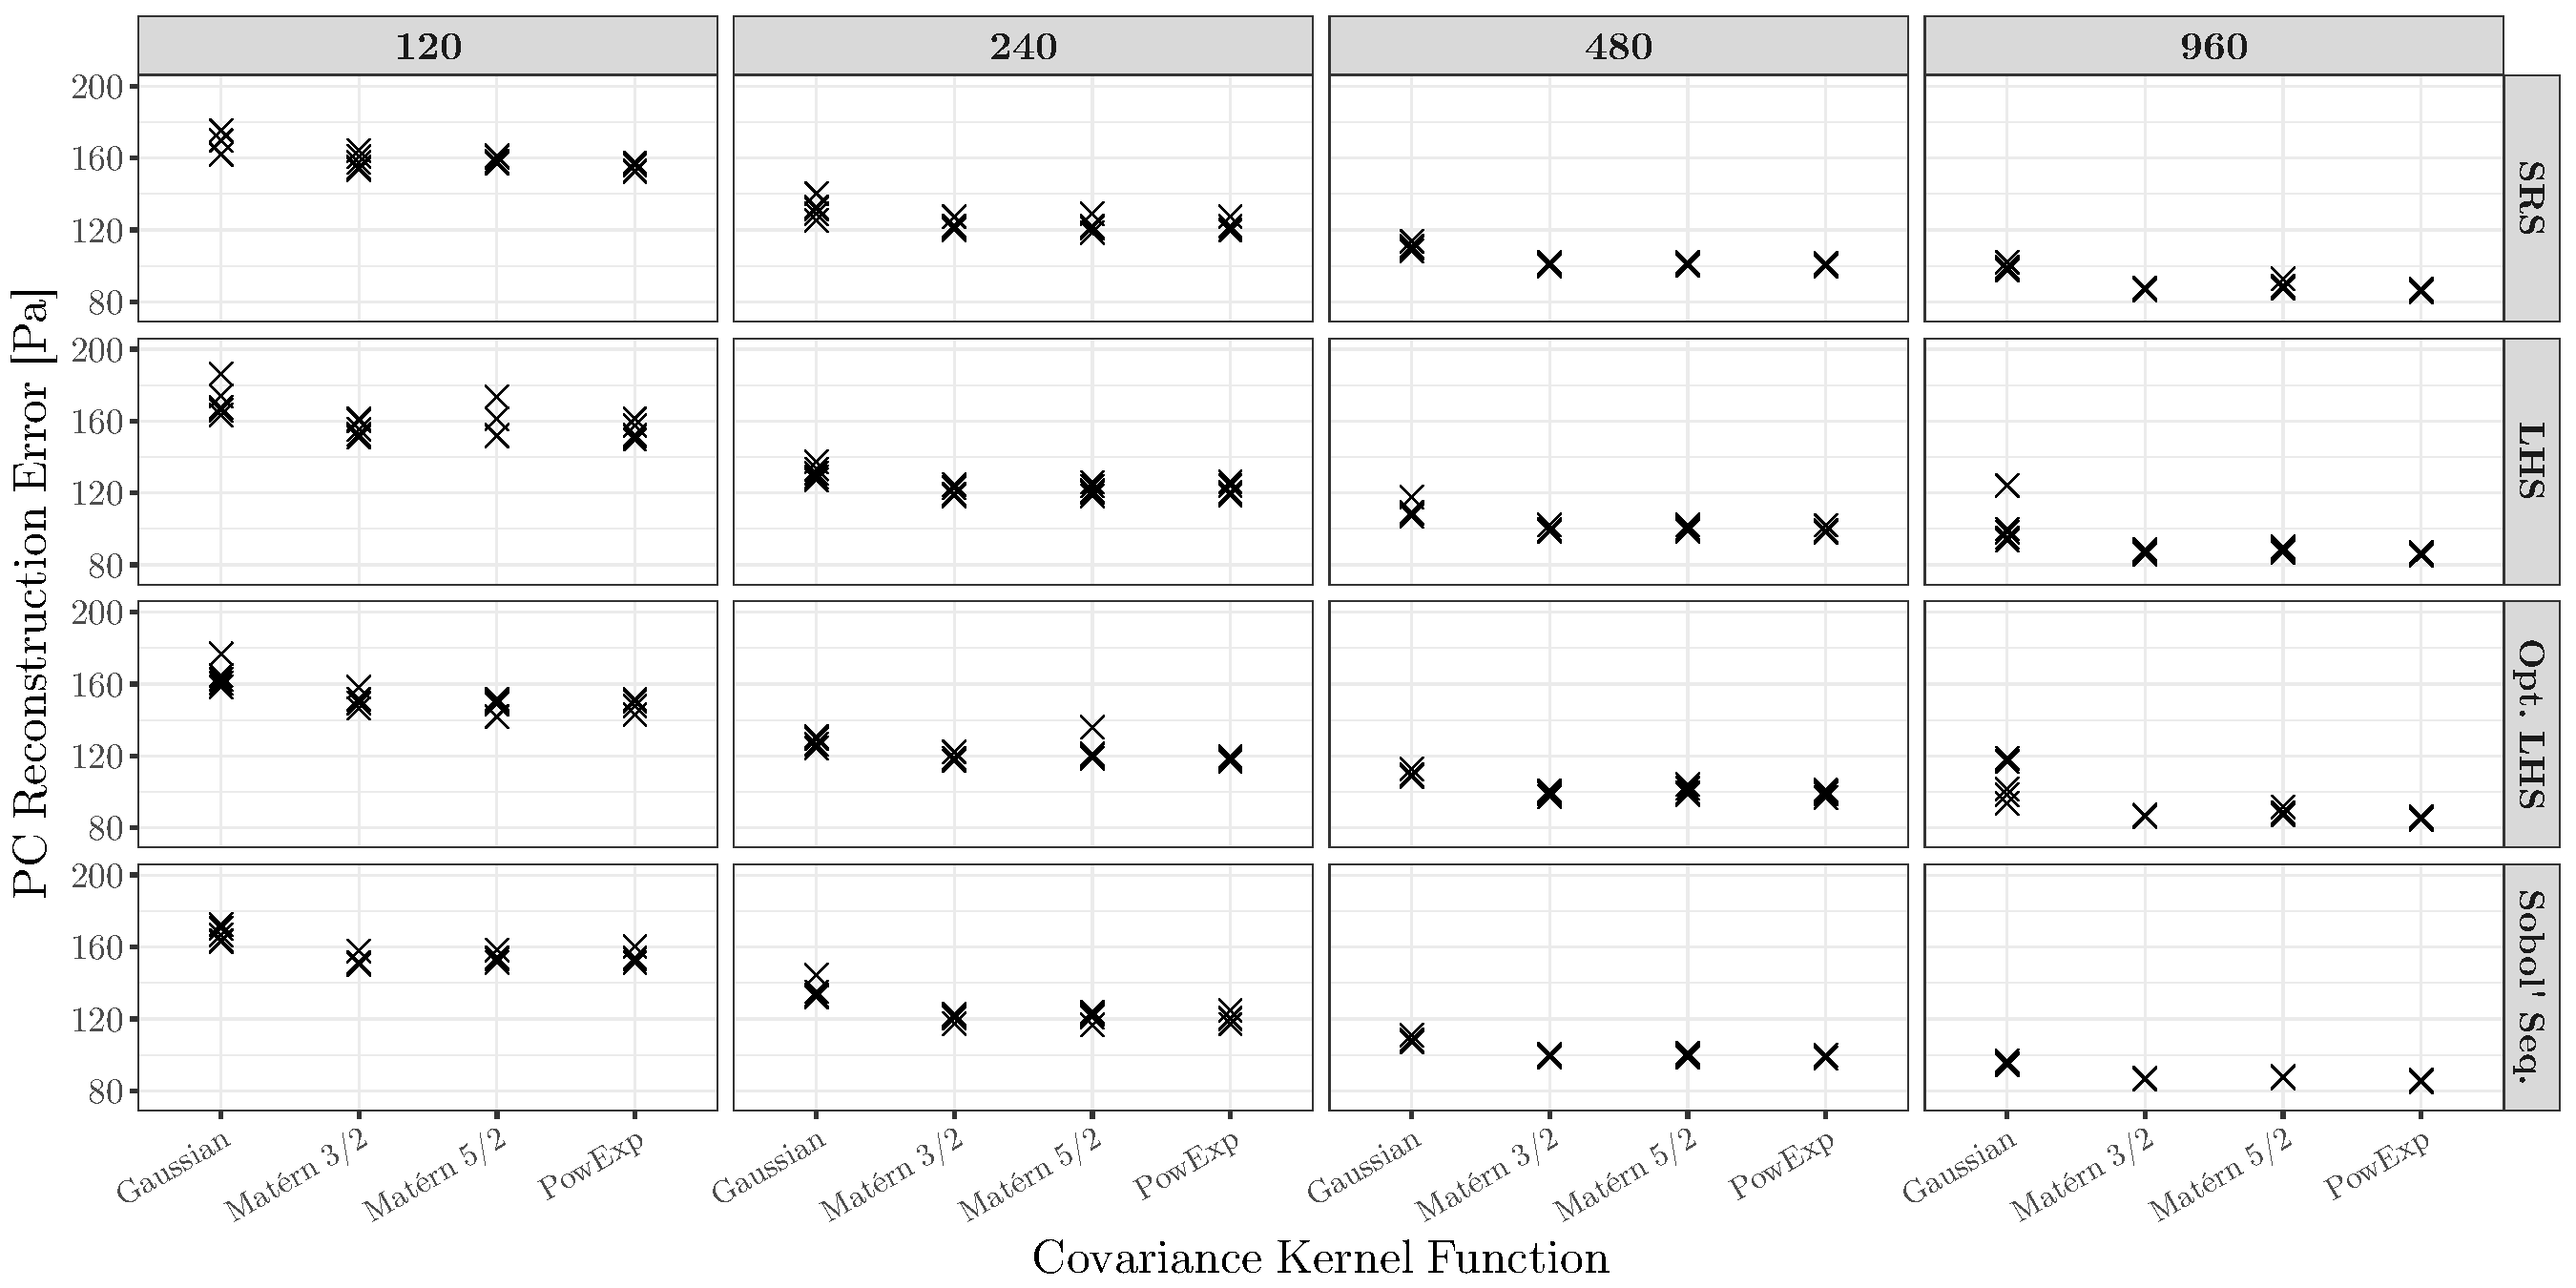
\includegraphics[width=1.0\textwidth]{../figures/chapter4/figures/plotPCGPConstructionDP}
	\caption[The effect of training sample size, experimental design, and covariance function on the predictive performance of GP PC metamodel with respect to the pressure drop output]{The effect of training sample size, experimental design, and covariance function on the predictive performance (in terms of \gls[hyper=false]{rmse}, of \gls[hyper=false]{gp} \gls[hyper=false]{pc} metamodel with respect to the pressure drop output.}
	\label{fig:ch4_plot_pc_gp_construction_dp}
\end{sidewaysfigure}
\clearpage

% PC GP Metamodel Construction, Liquid Carryover output
\clearpage
\begin{sidewaysfigure}
	\centering
	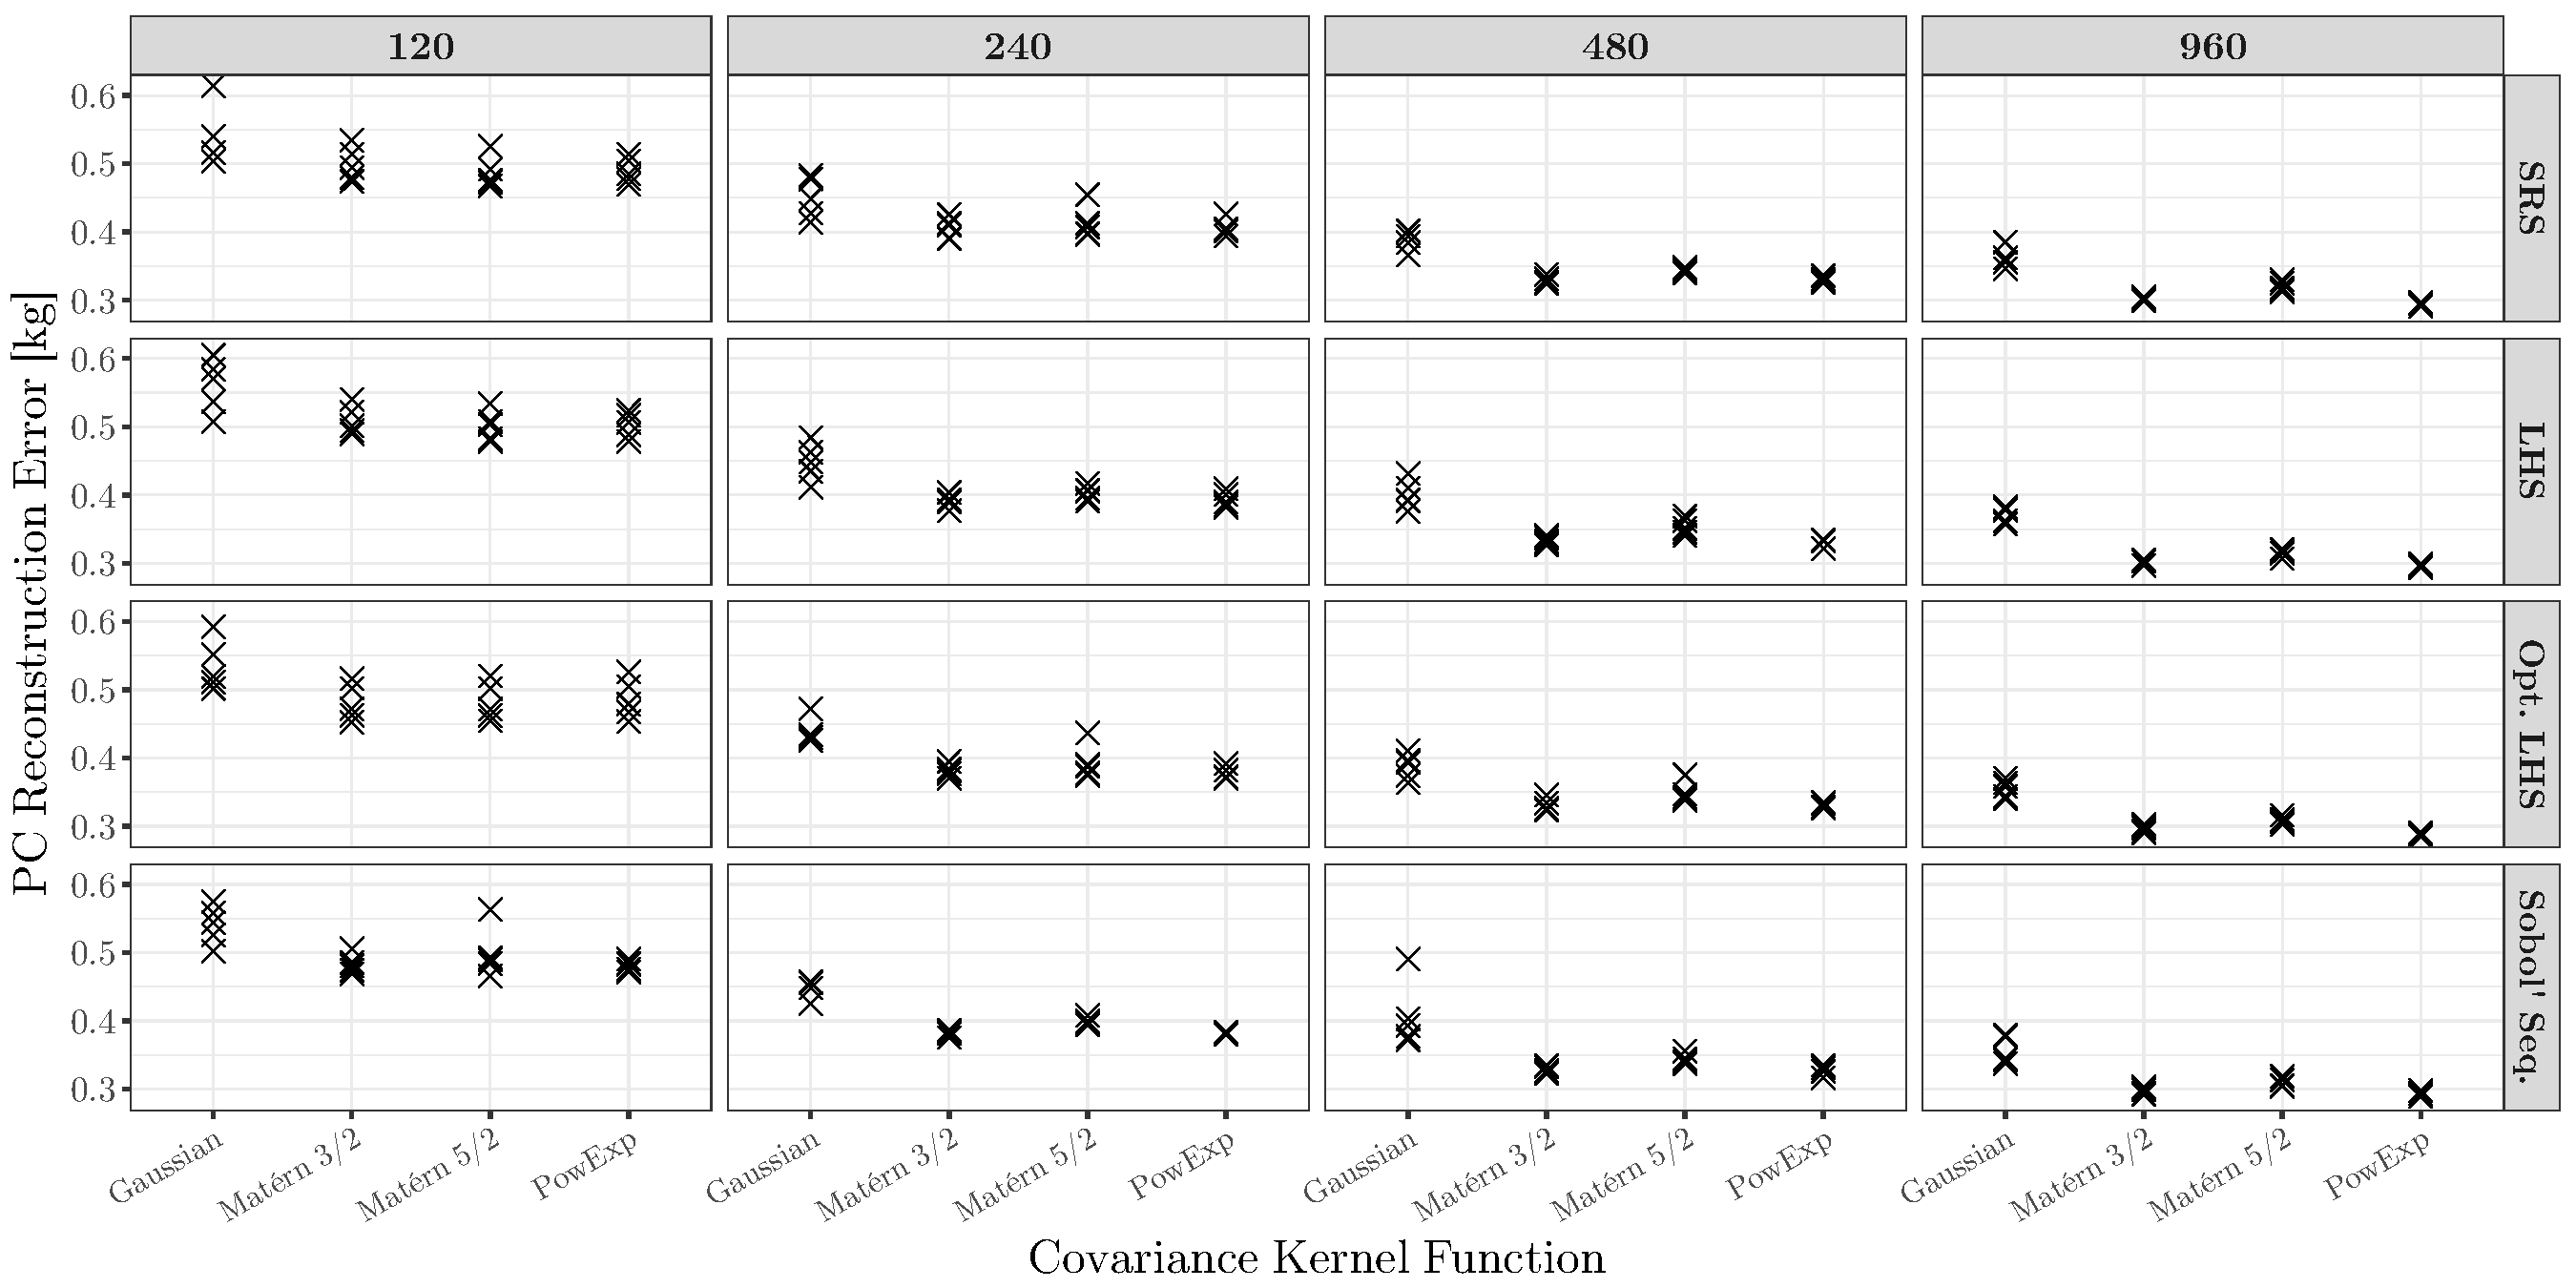
\includegraphics[width=1.0\textwidth]{../figures/chapter4/figures/plotPCGPConstructionCO}
	\caption[The effect of training sample size, experimental design, and covariance function on the predictive performance of GP PC metamodel with respect to the liquid carryover output]{The effect of training sample size, experimental design, and covariance function on the predictive performance (in terms of \gls[hyper=false]{rmse}, of \gls[hyper=false]{gp} \gls[hyper=false]{pc} metamodel with respect to the liquid carryover output.}
	\label{fig:ch4_plot_pc_gp_construction_co}
\end{sidewaysfigure}
\clearpage